\chapter{研究目的}
% 前述の通り、IJJ素子の特性を調べるため、40GHz以上で共振周波数の調整が可能な空洞共振器の設計が目的である。過去の研究成果を元に詳しい目標を整理する。

\section{昨年度の研究成果}
昨年度は、空洞共振器に誘電体を挿入した際の共振周波数の変化を調べていた
\cite{わたなべ}。Fig2.1に昨年度の計算結果を再現した結果を示す。
ここではmm,mm,mmの方形空洞を使用し、挿入した誘電体の誘電率は100、大きさはの円筒形、グラフに示されたhは誘電体の空洞内部への挿入長を示す。
その結果誘電体を挿入すると、共振周波数を減少できることがわかった。

\vspace{10 mm}

\begin{figure}[h]
  \begin{center}
    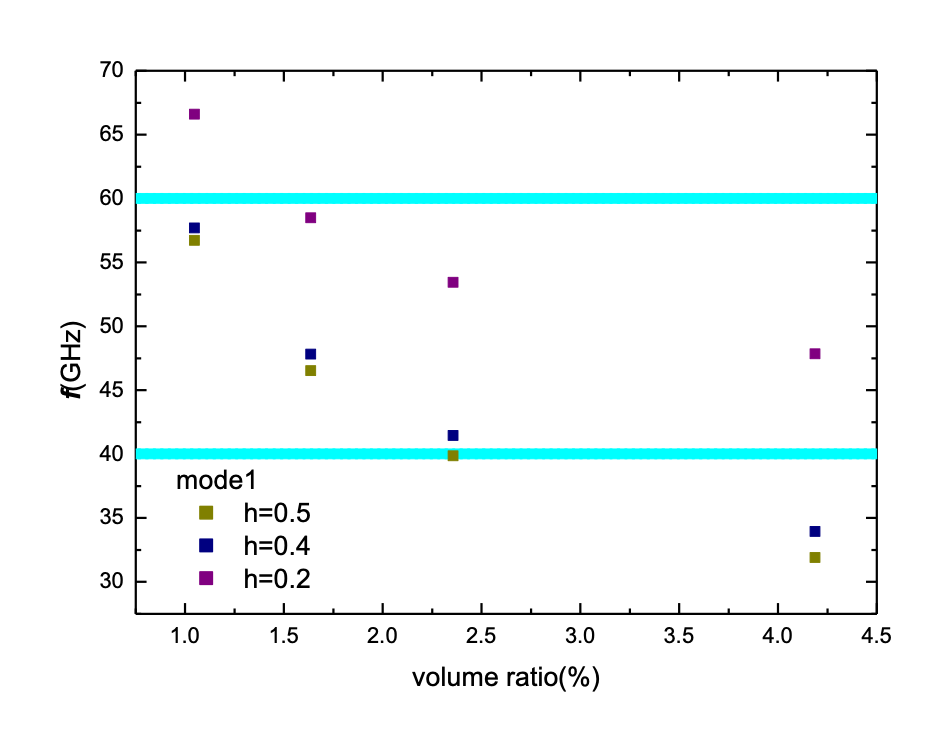
\includegraphics[width=12cm]{./image/watanabe.png}
    \caption{誘電体挿入時の共振周波数変化}
    \label{fig:Watanabe}
  \end{center}
\end{figure}

\section{昨年度の課題}
昨年度の研究\cite{わたなべ}では、
誘電体を挿入すると共振周波数が下がる効果が観測されたが、
以下の3点が不明瞭なため実用的な(実現可能な)モデルとは言えない。


\subsection*{共振周波数の調整方法}
昨年度使用していた誘電体の誘電率は100程度であり、
マイクロメータを使用して共振周波数を調整したとしても、
細かく共振周波数を制御できる仕様ではない。
また、シミュレーションの実施パターンが
共振器と誘電体の形状(方形か円筒形か)による違い
程度で検証数が少なく、
具体的な共振周波数調整方法が不明瞭であった。

\subsection*{外界との結合方法}
空洞共振器は単体で共振現象を起こすものではなく、
必ず外部からマイクロ波電力を入力し、
外界の入力電磁場と共振モードの電磁場を互いに結合する必要がある。
本研究では、外界と共振器の電磁場を結合させるために
外形約2.2mmの同軸ケーブルを使用する。
これに対し、昨年度のモデルでは、
空洞の一辺の長さが1mm程度であり、
直径が2mm程度の同軸ケーブルでは接続することができず結合方法が不明瞭であった。

\subsection*{試料の設置位置}
試料(超伝導量子ビットを実装するジョセフソン接合)の設置位置は、
空洞共振器内部の電場分布から決定するが、
昨年度の計算では、誘電体挿入時の分布が調べられていなかったため、
試料の設置位置も検討されていなかった。

\section{本研究の目的}
昨年度の研究成果を分析し、改めて整理すると、

\begin{itemize}
  \item 誘電体挿入による共振周波数変化の定量性
  \item 同軸ケーブルとの接続
  \item 誘電体挿入時の電場変化を考慮した試料位置の決定
\end{itemize}

の3点を新たに満たし、
共振周波数が40GHz以上で調整できる
実用的な空洞共振器の設計を行うことべきであるという方針が得られた。
したがって本研究の目標は上記3点を満たし、試作器による実験実施に向けた空洞共振器を
次章でシエmす電磁界解析シミュレーターを用いて設計することである。
% また、調整精度に関しては現時点では不明であるため、
